% Options for packages loaded elsewhere
\PassOptionsToPackage{unicode}{hyperref}
\PassOptionsToPackage{hyphens}{url}
%
\documentclass[
  10pt,
  b5paper,
  oneside]{book}
\usepackage{amsmath,amssymb}
\usepackage{lmodern}
\usepackage{iftex}
\ifPDFTeX
  \usepackage[T1]{fontenc}
  \usepackage[utf8]{inputenc}
  \usepackage{textcomp} % provide euro and other symbols
\else % if luatex or xetex
  \usepackage{unicode-math}
  \defaultfontfeatures{Scale=MatchLowercase}
  \defaultfontfeatures[\rmfamily]{Ligatures=TeX,Scale=1}
\fi
% Use upquote if available, for straight quotes in verbatim environments
\IfFileExists{upquote.sty}{\usepackage{upquote}}{}
\IfFileExists{microtype.sty}{% use microtype if available
  \usepackage[]{microtype}
  \UseMicrotypeSet[protrusion]{basicmath} % disable protrusion for tt fonts
}{}
\makeatletter
\@ifundefined{KOMAClassName}{% if non-KOMA class
  \IfFileExists{parskip.sty}{%
    \usepackage{parskip}
  }{% else
    \setlength{\parindent}{0pt}
    \setlength{\parskip}{6pt plus 2pt minus 1pt}}
}{% if KOMA class
  \KOMAoptions{parskip=half}}
\makeatother
\usepackage{xcolor}
\usepackage{color}
\usepackage{fancyvrb}
\newcommand{\VerbBar}{|}
\newcommand{\VERB}{\Verb[commandchars=\\\{\}]}
\DefineVerbatimEnvironment{Highlighting}{Verbatim}{commandchars=\\\{\}}
% Add ',fontsize=\small' for more characters per line
\usepackage{framed}
\definecolor{shadecolor}{RGB}{248,248,248}
\newenvironment{Shaded}{\begin{snugshade}}{\end{snugshade}}
\newcommand{\AlertTok}[1]{\textcolor[rgb]{0.94,0.16,0.16}{#1}}
\newcommand{\AnnotationTok}[1]{\textcolor[rgb]{0.56,0.35,0.01}{\textbf{\textit{#1}}}}
\newcommand{\AttributeTok}[1]{\textcolor[rgb]{0.77,0.63,0.00}{#1}}
\newcommand{\BaseNTok}[1]{\textcolor[rgb]{0.00,0.00,0.81}{#1}}
\newcommand{\BuiltInTok}[1]{#1}
\newcommand{\CharTok}[1]{\textcolor[rgb]{0.31,0.60,0.02}{#1}}
\newcommand{\CommentTok}[1]{\textcolor[rgb]{0.56,0.35,0.01}{\textit{#1}}}
\newcommand{\CommentVarTok}[1]{\textcolor[rgb]{0.56,0.35,0.01}{\textbf{\textit{#1}}}}
\newcommand{\ConstantTok}[1]{\textcolor[rgb]{0.00,0.00,0.00}{#1}}
\newcommand{\ControlFlowTok}[1]{\textcolor[rgb]{0.13,0.29,0.53}{\textbf{#1}}}
\newcommand{\DataTypeTok}[1]{\textcolor[rgb]{0.13,0.29,0.53}{#1}}
\newcommand{\DecValTok}[1]{\textcolor[rgb]{0.00,0.00,0.81}{#1}}
\newcommand{\DocumentationTok}[1]{\textcolor[rgb]{0.56,0.35,0.01}{\textbf{\textit{#1}}}}
\newcommand{\ErrorTok}[1]{\textcolor[rgb]{0.64,0.00,0.00}{\textbf{#1}}}
\newcommand{\ExtensionTok}[1]{#1}
\newcommand{\FloatTok}[1]{\textcolor[rgb]{0.00,0.00,0.81}{#1}}
\newcommand{\FunctionTok}[1]{\textcolor[rgb]{0.00,0.00,0.00}{#1}}
\newcommand{\ImportTok}[1]{#1}
\newcommand{\InformationTok}[1]{\textcolor[rgb]{0.56,0.35,0.01}{\textbf{\textit{#1}}}}
\newcommand{\KeywordTok}[1]{\textcolor[rgb]{0.13,0.29,0.53}{\textbf{#1}}}
\newcommand{\NormalTok}[1]{#1}
\newcommand{\OperatorTok}[1]{\textcolor[rgb]{0.81,0.36,0.00}{\textbf{#1}}}
\newcommand{\OtherTok}[1]{\textcolor[rgb]{0.56,0.35,0.01}{#1}}
\newcommand{\PreprocessorTok}[1]{\textcolor[rgb]{0.56,0.35,0.01}{\textit{#1}}}
\newcommand{\RegionMarkerTok}[1]{#1}
\newcommand{\SpecialCharTok}[1]{\textcolor[rgb]{0.00,0.00,0.00}{#1}}
\newcommand{\SpecialStringTok}[1]{\textcolor[rgb]{0.31,0.60,0.02}{#1}}
\newcommand{\StringTok}[1]{\textcolor[rgb]{0.31,0.60,0.02}{#1}}
\newcommand{\VariableTok}[1]{\textcolor[rgb]{0.00,0.00,0.00}{#1}}
\newcommand{\VerbatimStringTok}[1]{\textcolor[rgb]{0.31,0.60,0.02}{#1}}
\newcommand{\WarningTok}[1]{\textcolor[rgb]{0.56,0.35,0.01}{\textbf{\textit{#1}}}}
\usepackage{longtable,booktabs,array}
\usepackage{calc} % for calculating minipage widths
% Correct order of tables after \paragraph or \subparagraph
\usepackage{etoolbox}
\makeatletter
\patchcmd\longtable{\par}{\if@noskipsec\mbox{}\fi\par}{}{}
\makeatother
% Allow footnotes in longtable head/foot
\IfFileExists{footnotehyper.sty}{\usepackage{footnotehyper}}{\usepackage{footnote}}
\makesavenoteenv{longtable}
\usepackage{graphicx}
\makeatletter
\def\maxwidth{\ifdim\Gin@nat@width>\linewidth\linewidth\else\Gin@nat@width\fi}
\def\maxheight{\ifdim\Gin@nat@height>\textheight\textheight\else\Gin@nat@height\fi}
\makeatother
% Scale images if necessary, so that they will not overflow the page
% margins by default, and it is still possible to overwrite the defaults
% using explicit options in \includegraphics[width, height, ...]{}
\setkeys{Gin}{width=\maxwidth,height=\maxheight,keepaspectratio}
% Set default figure placement to htbp
\makeatletter
\def\fps@figure{htbp}
\makeatother
\setlength{\emergencystretch}{3em} % prevent overfull lines
\providecommand{\tightlist}{%
  \setlength{\itemsep}{0pt}\setlength{\parskip}{0pt}}
\setcounter{secnumdepth}{5}
\newlength{\cslhangindent}
\setlength{\cslhangindent}{1.5em}
\newlength{\csllabelwidth}
\setlength{\csllabelwidth}{3em}
\newlength{\cslentryspacingunit} % times entry-spacing
\setlength{\cslentryspacingunit}{\parskip}
\newenvironment{CSLReferences}[2] % #1 hanging-ident, #2 entry spacing
 {% don't indent paragraphs
  \setlength{\parindent}{0pt}
  % turn on hanging indent if param 1 is 1
  \ifodd #1
  \let\oldpar\par
  \def\par{\hangindent=\cslhangindent\oldpar}
  \fi
  % set entry spacing
  \setlength{\parskip}{#2\cslentryspacingunit}
 }%
 {}
\usepackage{calc}
\newcommand{\CSLBlock}[1]{#1\hfill\break}
\newcommand{\CSLLeftMargin}[1]{\parbox[t]{\csllabelwidth}{#1}}
\newcommand{\CSLRightInline}[1]{\parbox[t]{\linewidth - \csllabelwidth}{#1}\break}
\newcommand{\CSLIndent}[1]{\hspace{\cslhangindent}#1}
\usepackage{booktabs}
\usepackage{amsthm}
\makeatletter
\let\stdl@chapter\l@chapter
\renewcommand*{\l@chapter}[2]{%
  \stdl@chapter{\textcolor{astral}{#1}}{\textcolor{astral}{#2}}}

\def\thm@space@setup{%
  \thm@preskip=5cm
  \thm@postskip=\thm@preskip

}
\usepackage{graphicx}
\usepackage{afterpage}

\newcommand\blankpage{%
    \null
    \thispagestyle{empty}%
    \addtocounter{page}{-1}%
    \newpage}

\usepackage{amssymb}
\usepackage{amsmath}
%\pagestyle{plain} % default for report

\usepackage{etoolbox}
\makeatletter
\patchcmd{\@makechapterhead}{50\p@}{-24pt}{}{}
\patchcmd{\@makeschapterhead}{50\p@}{-24pt}{}{}
\makeatother

\makeatother
\usepackage{sectsty}

\definecolor{astral}{RGB}{153, 61, 15}
\allsectionsfont{\sffamily\color{astral}}


\usepackage{fancyhdr}
\usepackage{pdfpages}

\renewcommand{\headrulewidth}{0.5pt}
\renewcommand{\headrule}{\hbox to\headwidth{\color{astral}\leaders\hrule height \headrulewidth\hfill}}


\setlength{\headheight}{5pt}

\fancyhf{}
\fancyhead[EL]{\nouppercase\leftmark}
\fancyhead[OR]{\nouppercase\rightmark}
\fancyhead[ER,OL]{\thepage}

\usepackage{multicol}
\usepackage{hyperref}
\usepackage{longtable}
\usepackage{array}
\usepackage{multirow}
\usepackage{wrapfig}
\usepackage{float}
\usepackage{colortbl}
\usepackage{pdflscape}
\usepackage{tabu}
\usepackage{threeparttable}
\usepackage{adjustbox}
\usepackage{rotating}
\usepackage{tablefootnote}
\usepackage[normalem]{ulem}
% empty pages betwen chapters
\usepackage{emptypage}


\makeatletter
\makeatother

\renewcommand{\listfigurename}{Figures}
\renewcommand{\listtablename}{Tables}

\usepackage[sectionbib]{chapterbib}

%% List of Abbreviations
\usepackage{nomencl}
\makenomenclature
\renewcommand{\nomname}{Acronyms}
%% to update run makeindex on docs folder and move results to / folder
%% see nomencl manual
%% e.g. makeindex SOCMapping.nlo -s nomencl.ist -o SOCMapping.nls

%% index
\usepackage{imakeidx}
\makeindex

\usepackage{xspace}

% no title page
\AtBeginDocument{\let\maketitle\relax}
\hypersetup{
	colorlinks=true,
	linkcolor=astral,
	filecolor=astral,
	urlcolor=astral,
	citecolor=astral
}
\AtBeginDocument{\renewcommand{\chaptername}{Chapter}}
\usepackage{titling}
\usepackage{natbib}
\usepackage{pdfpages}
\usepackage{fancyhdr}
\usepackage{booktabs}
\usepackage{longtable}
\usepackage{subfig}
\usepackage{array}
\usepackage{amsmath}
\usepackage{multirow}
\usepackage{wrapfig}
\usepackage{bookmark}
\usepackage[utf8]{inputenc}
\usepackage{float}
\usepackage{colortbl}
\usepackage{pdflscape}
\usepackage{tabu}
\usepackage{threeparttable}
\usepackage{threeparttablex}
\usepackage[normalem]{ulem}
\usepackage{makecell}
\usepackage{xcolor}
\DeclareUnicodeCharacter{2212}{\textendash}
\usepackage{rotating, graphicx}
\ifLuaTeX
  \usepackage{selnolig}  % disable illegal ligatures
\fi
\IfFileExists{bookmark.sty}{\usepackage{bookmark}}{\usepackage{hyperref}}
\IfFileExists{xurl.sty}{\usepackage{xurl}}{} % add URL line breaks if available
\urlstyle{same} % disable monospaced font for URLs
\hypersetup{
  pdftitle={Digital Soil Mapping Technical Manual},
  pdfauthor={GSP Secretariat and ITPS},
  hidelinks,
  pdfcreator={LaTeX via pandoc}}

\title{Digital Soil Mapping Technical Manual}
\author{GSP Secretariat and ITPS}
\date{}

\begin{document}
\maketitle

\pagestyle{plain}
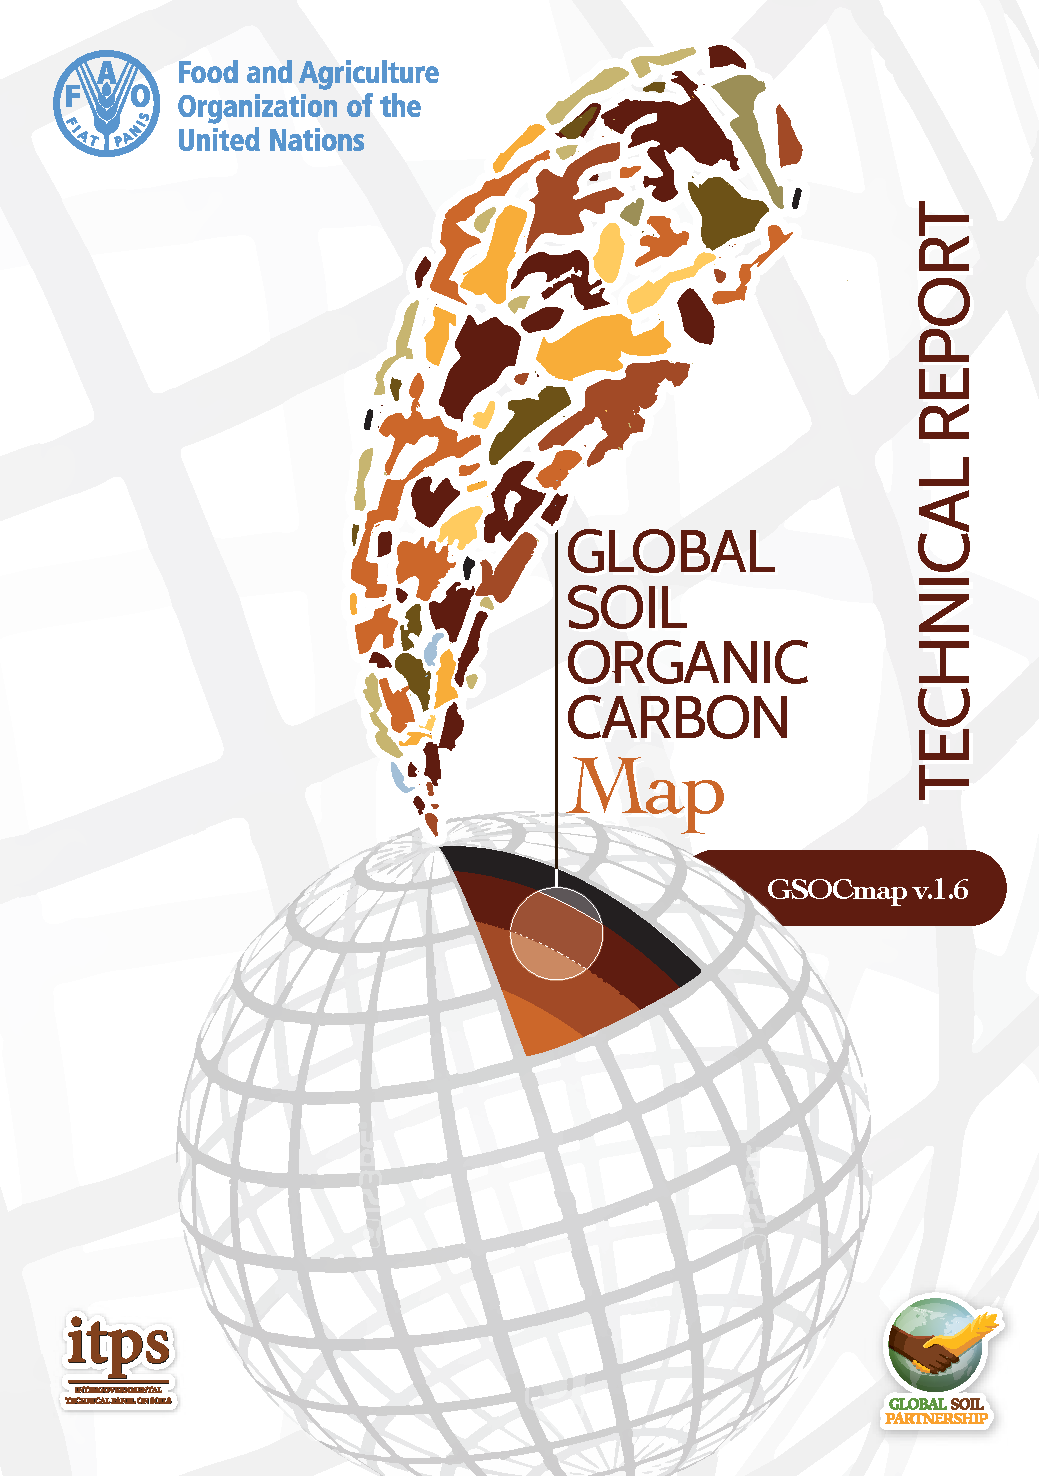
\includepdf{images/cover_1.6.pdf}
\afterpage{\blankpage}
\thispagestyle{empty}
\begin{titlepage}
    \begin{center}
        \vspace*{4cm}
        \Large

        \textcolor{astral}{\textbf{Country Guidelines on Digital Soil Mapping\\}}
        \vspace{0.5cm}
        \normalsize
        \vfill
        \noindent
        {\color{astral}\rule{\linewidth}{0.5mm} }

        Food and Agriculture Organization of the United Nations\\
	Rome, 2022
    \end{center}
\end{titlepage}
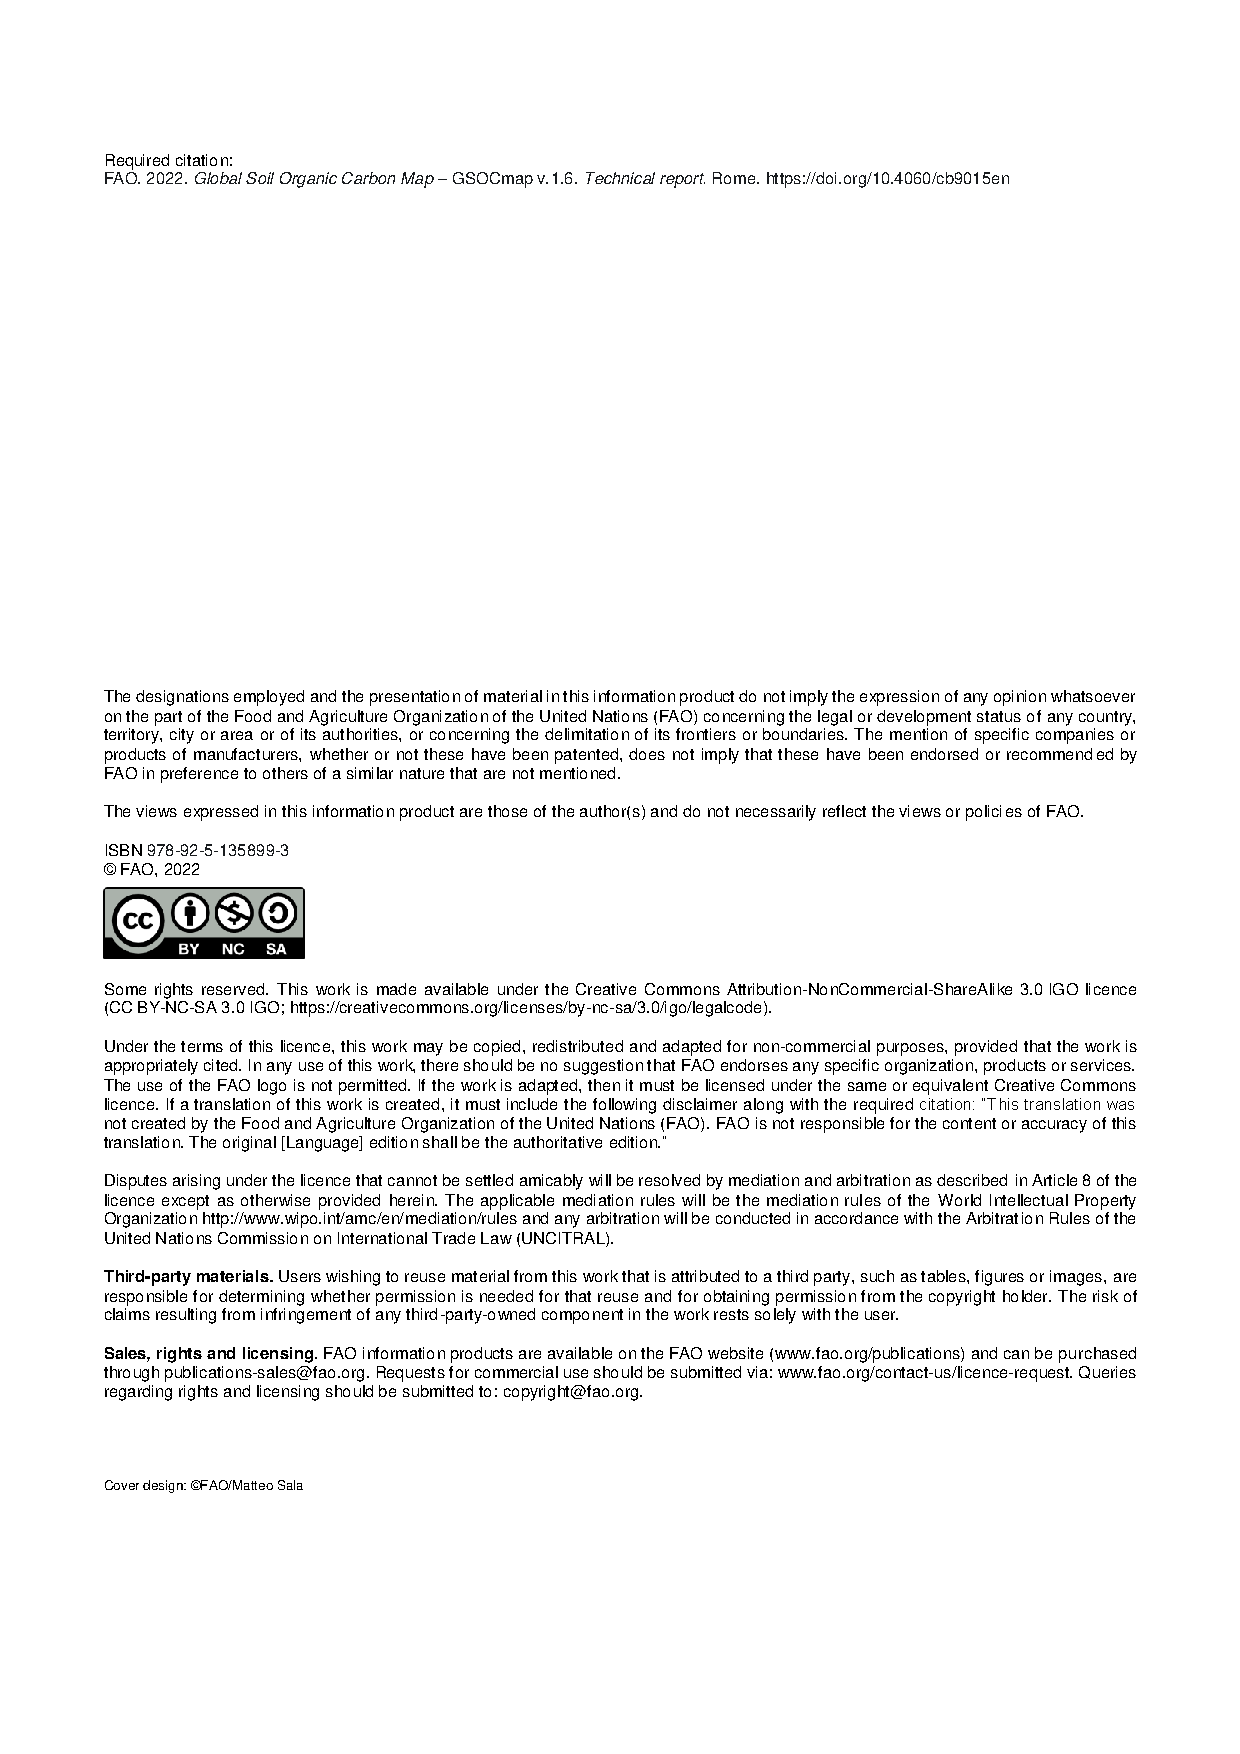
\includepdf{images/CB9015EN_Copyright Disclaimer_v2.pdf}


\frontmatter
\addtocontents{toc}{\protect\hypersetup{hidelinks}}   
\addtocontents{lof}{\protect\hypersetup{hidelinks}}
\addtocontents{lot}{\protect\hypersetup{hidelinks}}
\tableofcontents
\listoffigures
\listoftables
\nopagebreak[4]

\hypertarget{foreword}{%
\chapter*{Foreword}\label{foreword}}
\addcontentsline{toc}{chapter}{Foreword}

\hypertarget{abbreviations-and-acronyms}{%
\chapter*{Abbreviations and acronyms}\label{abbreviations-and-acronyms}}
\addcontentsline{toc}{chapter}{Abbreviations and acronyms}

\begin{description}
\item[BD]
Bulk Density
\item[CO\textsubscript{2}]
Carbon dioxide
\item[CRF]
Coarse fragments
\item[DM]
Dry matter
\item[DSM]
Digital soil mapping
\item[GAUL]
Global Administrative Unit Layers
\item[GHG]
Greenhouse gas
\item[GSOCmap]
Global Soil Organic Carbon Map
\item[GSOCseq]
Global Soil Organic Carbon Sequestration Potential Map
\item[GSP]
Global Soil Partnership
\item[HWSD]
Harmonized World Soil Database
\item[ISCN]
International Soil Carbon Network
\item[INSII]
International Network of Soil Information Institutions
\item[IPBES]
Intergovernmental Platform on Biodiversity and Ecosystem Services
\item[IPCC]
Intergovernmental Panel on Climate Change
\item[IPR]
Intellectual Property Rights
\item[ITPS]
Intergovernmental Technical Panel on Soils
\item[LDN]
Land Degradation Neutrality
\item[NDVI]
Normalized difference in vegetation index
\item[NPP]
Net Primary Production
\item[P4WG]
Pillar 4 Working Group
\item[QA/QC]
Quality Assurance/Quality Check
\item[RMSE]
Root mean square error
\item[SDF]
Soil Data Facility
\item[SDG]
Sustainable Development Goals
\item[SISLAC]
Latin America and the Caribbean's Soil Information System
\item[SOC]
Soil organic carbon
\item[SOM]
Soil organic matter
\item[SPADE/M]
Soil Profile Analytical Database of Europe of Measured Parameters
\item[SWRS]
Status of World's Soil Resources
\item[UNCCD]
United Nations Convention to Combat Desertification
\item[WFS]
Web Feature Service
\item[WoSIS]
World Soil Information Service
\end{description}

\hypertarget{contributors}{%
\chapter*{Contributors}\label{contributors}}
\addcontentsline{toc}{chapter}{Contributors}

\emph{Prepared by:}\\
\textbf{Global Soil Partnership Secretariat}\\
Ronald Vargas\\

\textbf{Second Intergovernmental Technical Panel on Soils}\\
Luca Montanarella - European Commission, Joint Research Centre
(\emph{Chair}); Saéb AbdelHaleem Khresat

\textbf{Third Intergovernmental Technical Panel on Soils}\\
Rosa Poch - Spain (\emph{Chair}); Nsalambi V. Nkongolo - Democratic Republic
of the Congo;

\mainmatter

\hypertarget{presentation}{%
\chapter{Presentation}\label{presentation}}

Soils provide ecosystem services critical to life on Earth. The Food and Agricultural Organization of the United Nations (FAO) recognizes the need to preserve soil resources from degradation and boost healthy soils. In 2012, FAO members established the Global Soil Partnership (GSP) as a mechanism to improve soil governance at global, regional and national levels\ldots{}

\hypertarget{setting-up-the-software-environment}{%
\chapter{Setting-up the software environment}\label{setting-up-the-software-environment}}

\emph{Y. Yigini}

This cookbook focuses on SOC modeling using open source digital mapping tools. The instructions in this chapter will guide the user through installing and manually configuring the software to be used for DSM procedures for Microsoft Windows desktop platform. Instructions for other platforms (e.g.~Linux Flavours, MacOS) can be found through free online resources.

\hypertarget{use-of-r-rstudio-and-r-packages}{%
\section{Use of R, RStudio and R Packages}\label{use-of-r-rstudio-and-r-packages}}

\textbf{R} is a language and environment for statistical computing. It provides a wide variety of statistical (e.g.~linear modeling, statistical tests, time-series, classification, clustering, etc.) and graphical methods, and is highly extensible.

\hypertarget{obtaining-and-installing-r}{%
\subsection{Obtaining and installing R}\label{obtaining-and-installing-r}}

Installation files and instructions can be downloaded from the Comprehensive R Archive Network (CRAN).

\begin{enumerate}
\def\labelenumi{\arabic{enumi}.}
\tightlist
\item
  Go to the following link \url{https://cran.r-project.org/} to download and install \textbf{R}.
\item
  Pick an installation file for your platform.
\end{enumerate}

\hypertarget{obtaining-and-installing-rstudio}{%
\subsection{Obtaining and installing RStudio}\label{obtaining-and-installing-rstudio}}

Beginners will find it very hard to start using \textbf{R} because it has no Graphical User Interface (GUI). There are some GUIs which offer some of the functionality of \textbf{R}. \textbf{RStudio} makes \textbf{R} easier to use. It includes a code editor, debugging and visualization tools. Similar steps need to be followed to install \textbf{RStudio}.

\begin{enumerate}
\def\labelenumi{\arabic{enumi}.}
\tightlist
\item
  Go to \url{https://www.rstudio.com/products/rstudio/download/} to download and install \textbf{RStudio}'s open source edition.
\item
  On the download page, \emph{RStudio Desktop, Open Source License} option should be selected.
\item
  Pick an installation file for your platform.
\end{enumerate}

\hypertarget{getting-started-with-r}{%
\subsection{Getting started with R}\label{getting-started-with-r}}

\begin{itemize}
\tightlist
\item
  \textbf{R} manuals: \url{http://cran.r-project.org/manuals.html}
\item
  Contributed documentation: \url{http://cran.r-project.org/other-docs.html}
\item
  Quick-\textbf{R}: \url{http://www.statmethods.net/index.html}
\item
  Stackoverflow \textbf{R} community: \url{https://stackoverflow.com/questions/tagged/r}
\end{itemize}

\hypertarget{r-packages}{%
\section{R packages}\label{r-packages}}

When you download \textbf{R}, you get the basic \textbf{R} system which implements the \textbf{R} language. \textbf{R} becomes more useful with the large collection of packages that extend the basic functionality of it. \textbf{R} packages are developed by the \textbf{R} community.

refer to:
- tidyverse book (R for data science)
- caret (cookbook)
- \url{https://rspatial.org/}

\hypertarget{finding-r-packages}{%
\subsection{Finding R packages}\label{finding-r-packages}}

The primary source for \textbf{R} packages is \href{https://cran.r-project.org/}{CRAN's} official website, where currently about 12,000 available packages are listed. For spatial applications, various packages are available. You can obtain information about the available packages directly on CRAN with the \texttt{available.packages()} function. The function returns a matrix of details corresponding to packages currently available at one or more repositories. An easier way to browse the list of packages is using the \href{https://cran.r-project.org/web/views/}{\emph{Task Views}} link, which groups together packages related to a given topic.

\hypertarget{gee---google-earth-engine}{%
\section{GEE - google earth engine}\label{gee---google-earth-engine}}

\begin{itemize}
\tightlist
\item
  general info
\end{itemize}

\begin{figure}
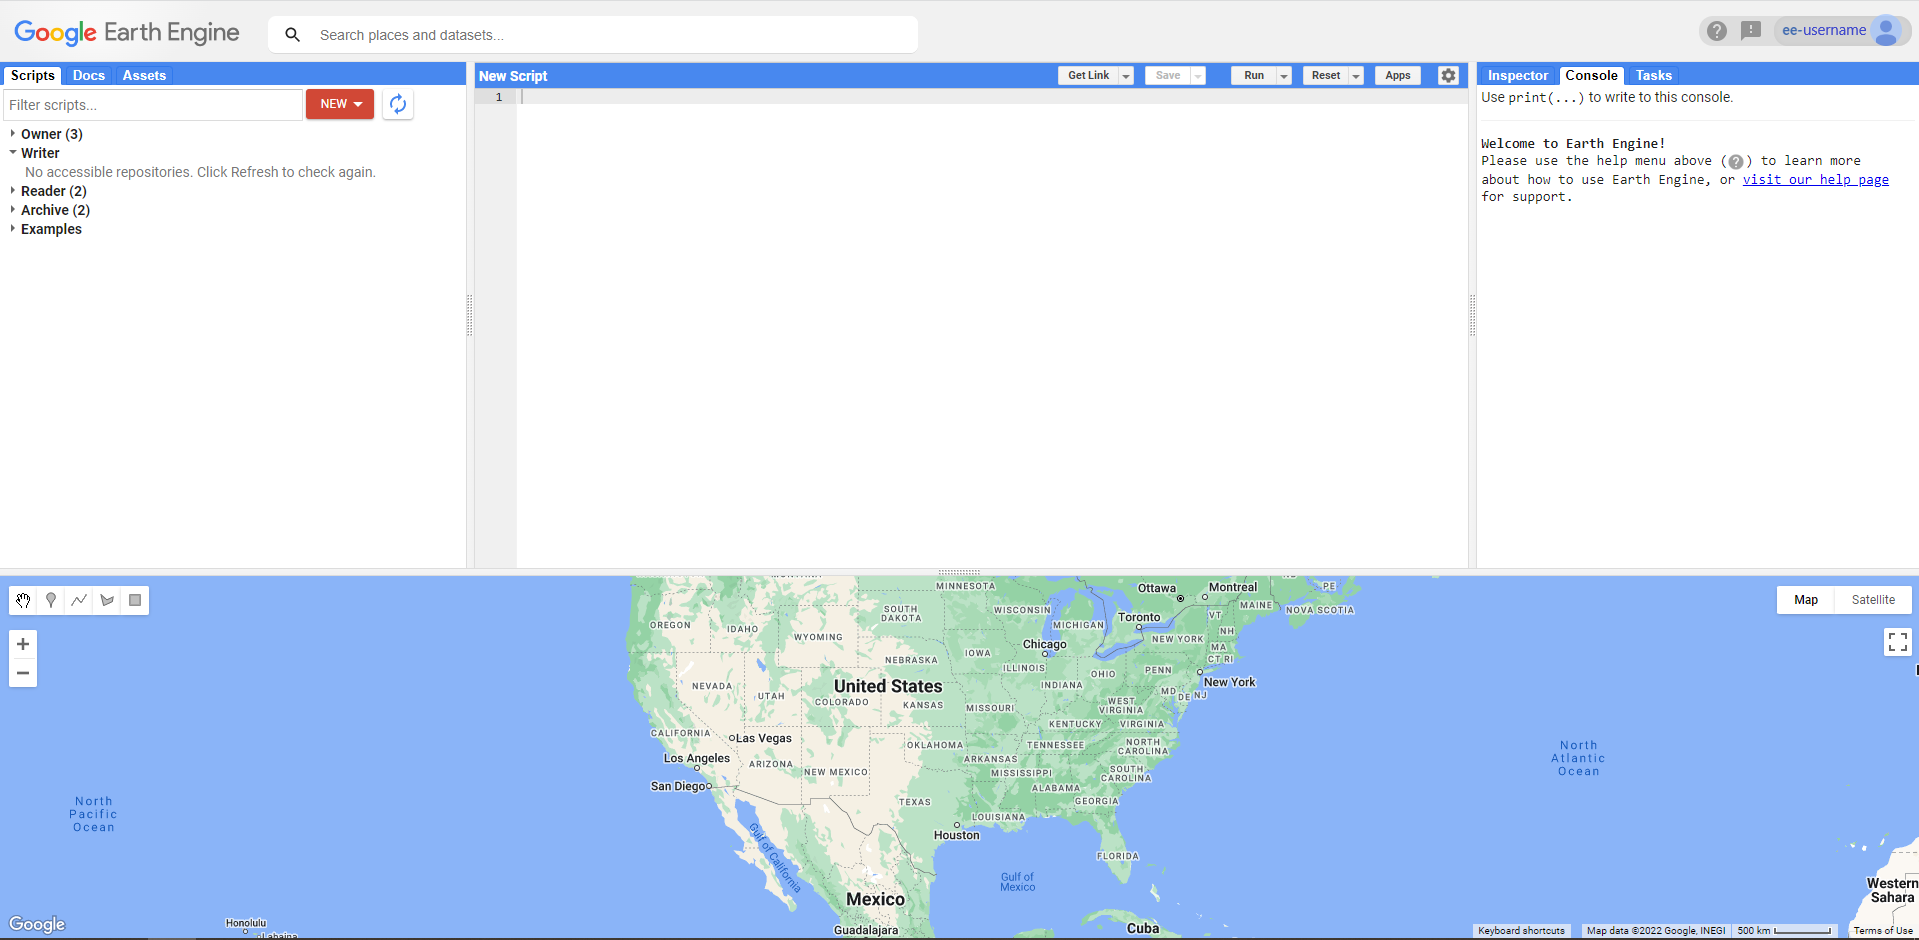
\includegraphics[width=12cm]{images/2.1_GEE_codeeditor} \caption{Google Earth Engine code editor.}\label{fig:unnamed-chunk-1}
\end{figure}

\begin{itemize}
\tightlist
\item
  upload assets to GEE
\end{itemize}

\begin{figure}
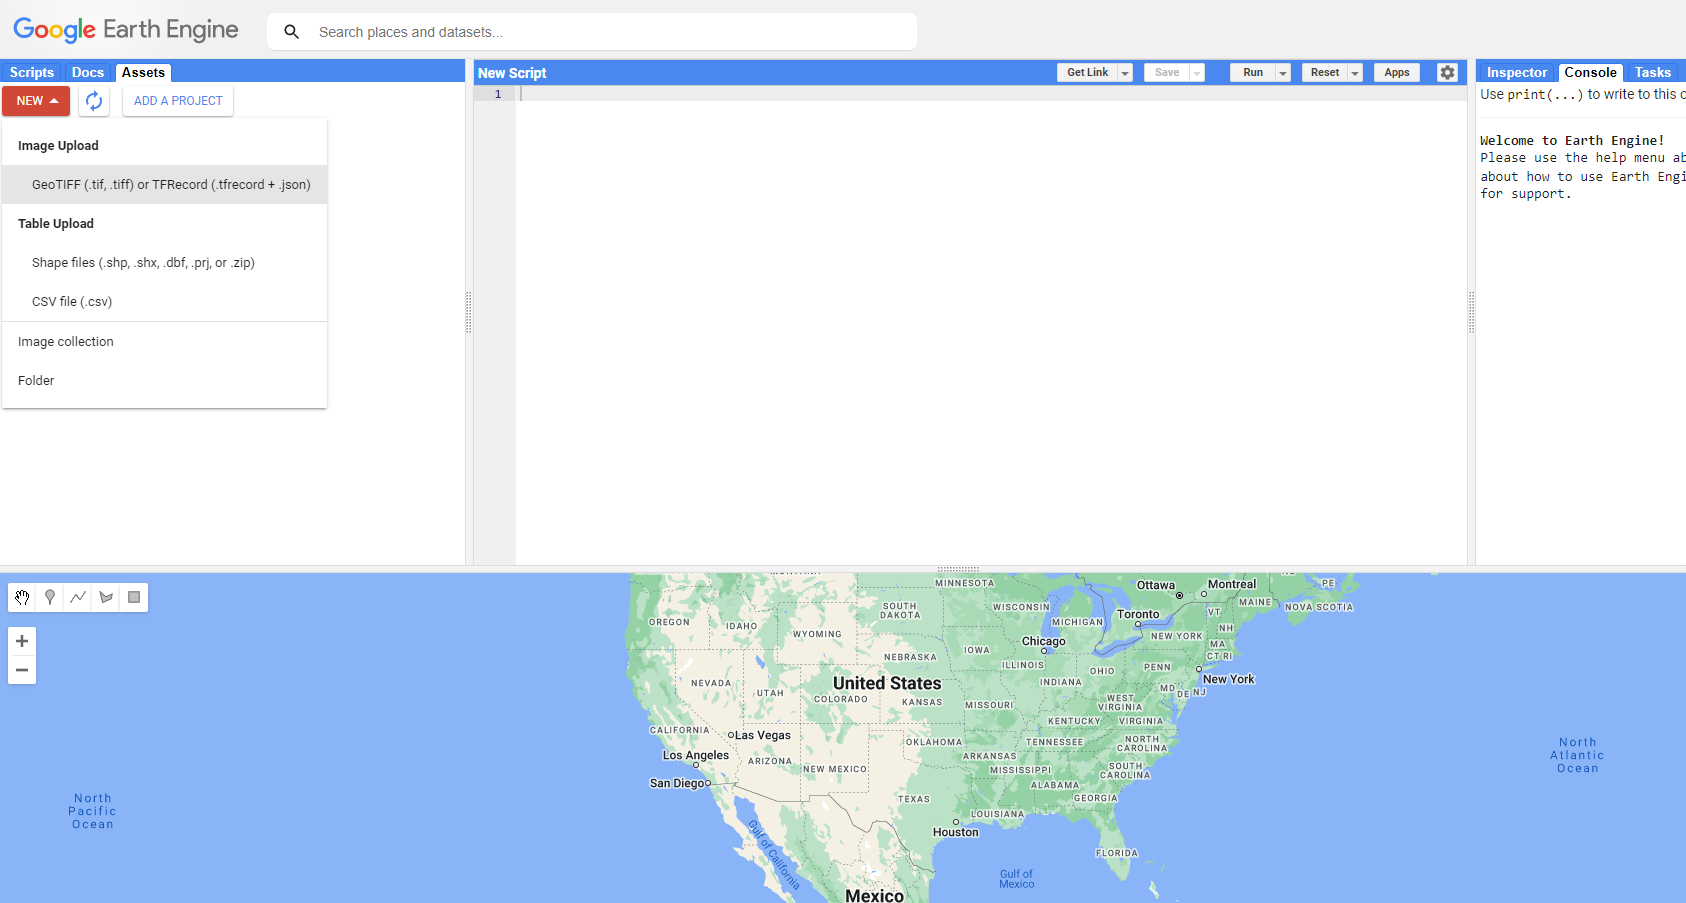
\includegraphics[width=12cm]{images/2.2_upload-assets-1} \caption{Select files and filetype to be uploaded as GEE assets.}\label{fig:unnamed-chunk-2}
\end{figure}

\begin{figure}
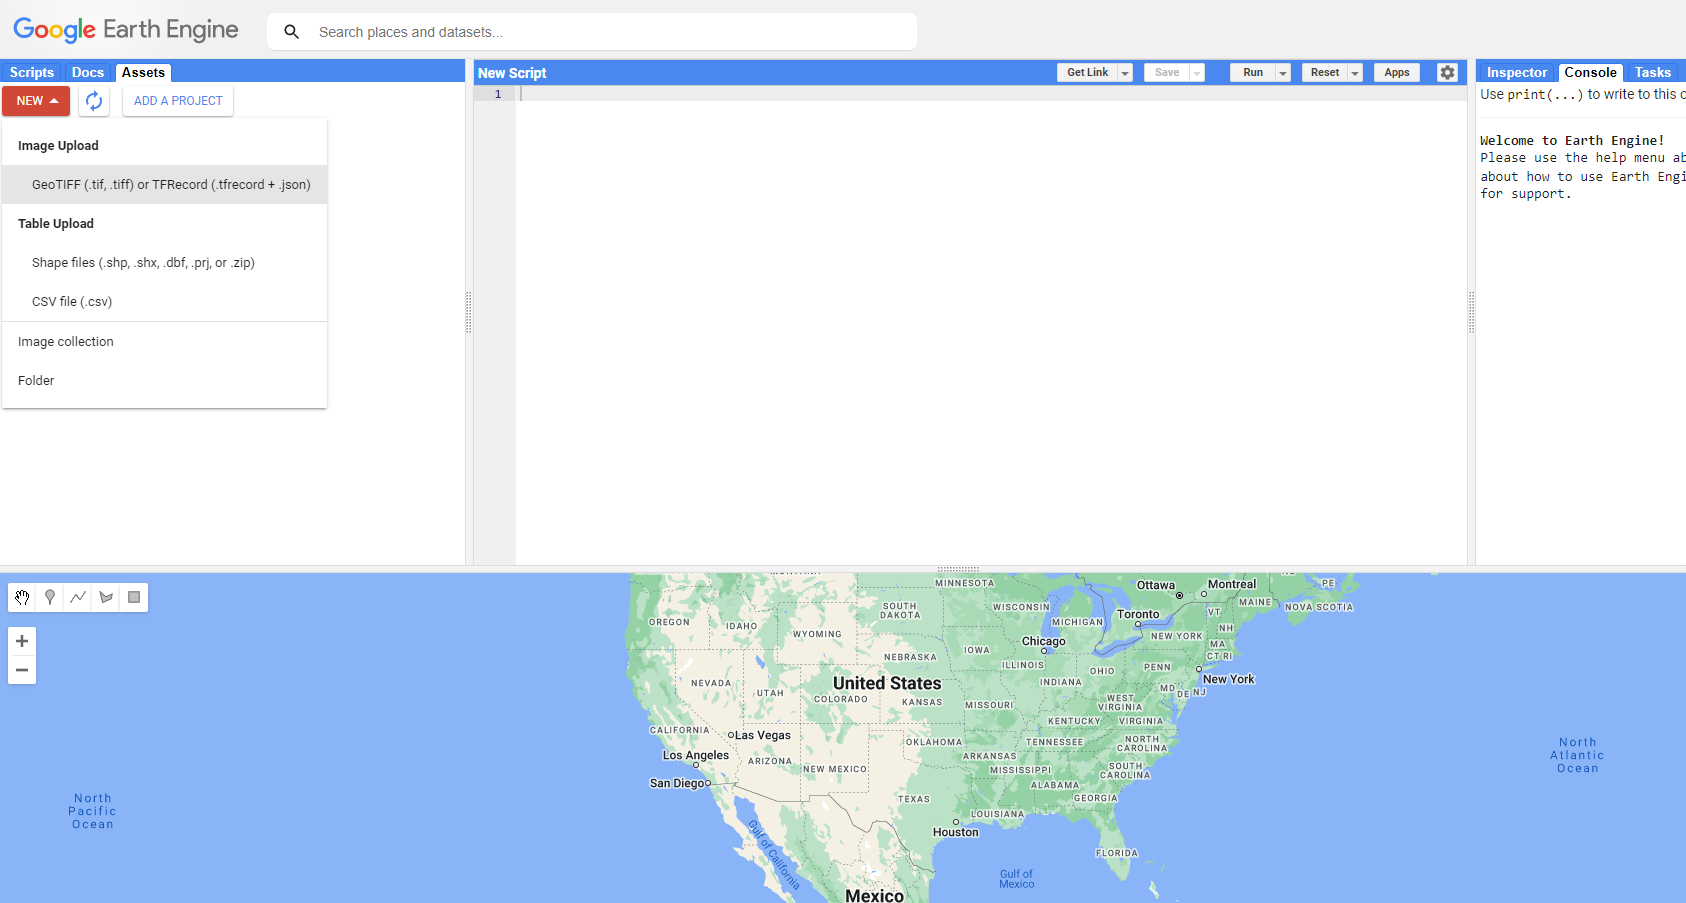
\includegraphics[width=12cm]{images/2.2_upload-assets-2} \caption{Upload interface.}\label{fig:unnamed-chunk-3}
\end{figure}

\begin{itemize}
\tightlist
\item
  Explain how to import uploaded assets (?) \ldots{}
\end{itemize}

\hypertarget{rgee---extension-to-use-google-earth-engine-in-r}{%
\section{rgee - Extension to use google earth engine in R}\label{rgee---extension-to-use-google-earth-engine-in-r}}

The rgee package enables users to interact with the GEE servers using the R language. The package makes use of the Python language to interact with GEE. The package can be downloaded easily either directly from the GitHub repository or via CRAN.

\begin{Shaded}
\begin{Highlighting}[]
\CommentTok{\# Source: https://yabellini.github.io/curso\_rgee/index.html}
\CommentTok{\# Yanina Bellini Saibene}

\CommentTok{\#install.packages(\textquotesingle{}remotes\textquotesingle{})}
\CommentTok{\# remotes::install\_github("r{-}spatial/rgee")}
\end{Highlighting}
\end{Shaded}

To be able to interact with the GEE via Python, it is necessary to install certain R packages but also the so-called ``Miniconda'' commmand prompt which acts as Python interpreter mediating between R and GEE. The `ee\_install()' function automatically downloads and install all the software that is needed.

\begin{Shaded}
\begin{Highlighting}[]
\CommentTok{\# load rgee package and install dependencies}
\FunctionTok{library}\NormalTok{(rgee)}
\CommentTok{\# ee\_install() \# installs miniconda}
\end{Highlighting}
\end{Shaded}

Once the dependencies are installed, it is necessary to initialize rgee by providing the user credentials of our GEE account. The ee\_Initialize command must be run every time we want to use rgee.

\begin{Shaded}
\begin{Highlighting}[]
\CommentTok{\# Initialize Google Earth Engine! (you need to create a user account)}
\CommentTok{\# ee\_Initialize()}


\CommentTok{\# Useful functions}

\CommentTok{\#ee\_check() \# check the dependencies that do not belong to R}
\CommentTok{\#ee\_clean\_credentials() \# to remove the user credentials}
\CommentTok{\#ee\_clean\_pyenv() \# Delete variables of the system}
\end{Highlighting}
\end{Shaded}

\hypertarget{introduction-to-digital-soil-mapping}{%
\chapter{Introduction to Digital Soil Mapping}\label{introduction-to-digital-soil-mapping}}

Digital soil mapping (DSM) is a methodological framework to create soil attribute maps on the basis of the quantitative relationships between spatial soil databases and environmental covariates. The quantitative relations can be modelled by different statistical approaches, most of them considered machine learning techniques. Environmental covariates are spatially explicit proxies of soil-forming factors that are employed as predictors of the geographical distribution of soil properties. The methodology has evolved from the theories of soil genesis developed by Vasil Dokuchaev in his work the Russian Chernozems (1883), which later were formalised by Jenny (1941) with the equation of the soil-forming factors. The conceptual equation of soil-forming factors has been updated by McBratney, Santos and Minasny (\protect\hyperlink{ref-McBratney2003}{2003}) as follow:

\begin{equation} 
  S = f\left(s,c,o,r,p,a,n\right)
  \label{eq:scorpan}
\end{equation}

Where \(S\) is the soil classes or attributes (to be modelled) as a function of ``\(s\)'' as other soil properties, ``\(c\)'' as climatic properties, ``\(o\)'' as organisms, including land cover and human activity, ``\(r\)'' as terrain attributes, ``\(p\)'' as parent material, ``\(a\)'' as soil age, and ``\(n\)'' as the geographic position.

Digital soil mapping has been used to produce maps of soil nutrients. For instance, Hengl \emph{et al.} (\protect\hyperlink{ref-Hengl2017}{2017}) predicted 15 soil nutrients at a 250 m resolution in Africa, using a random forest model (Wright and Ziegler, 2016), topsoil nutrient observations at point locations and a set of spatially-explicit environmental covariates. In 2021, Hengl et al.~applied the same modelling approach to estimate total phosphorus in semi-natural soils at the global scale, as well.

In this technical manual, we present a DSM frameworks to map soil properties, including soil nutrients. One approach for soil observations with latitude and longitude data (point-support) (Figure \ref{fig:workflow1}).

\begin{figure}
  \centering
  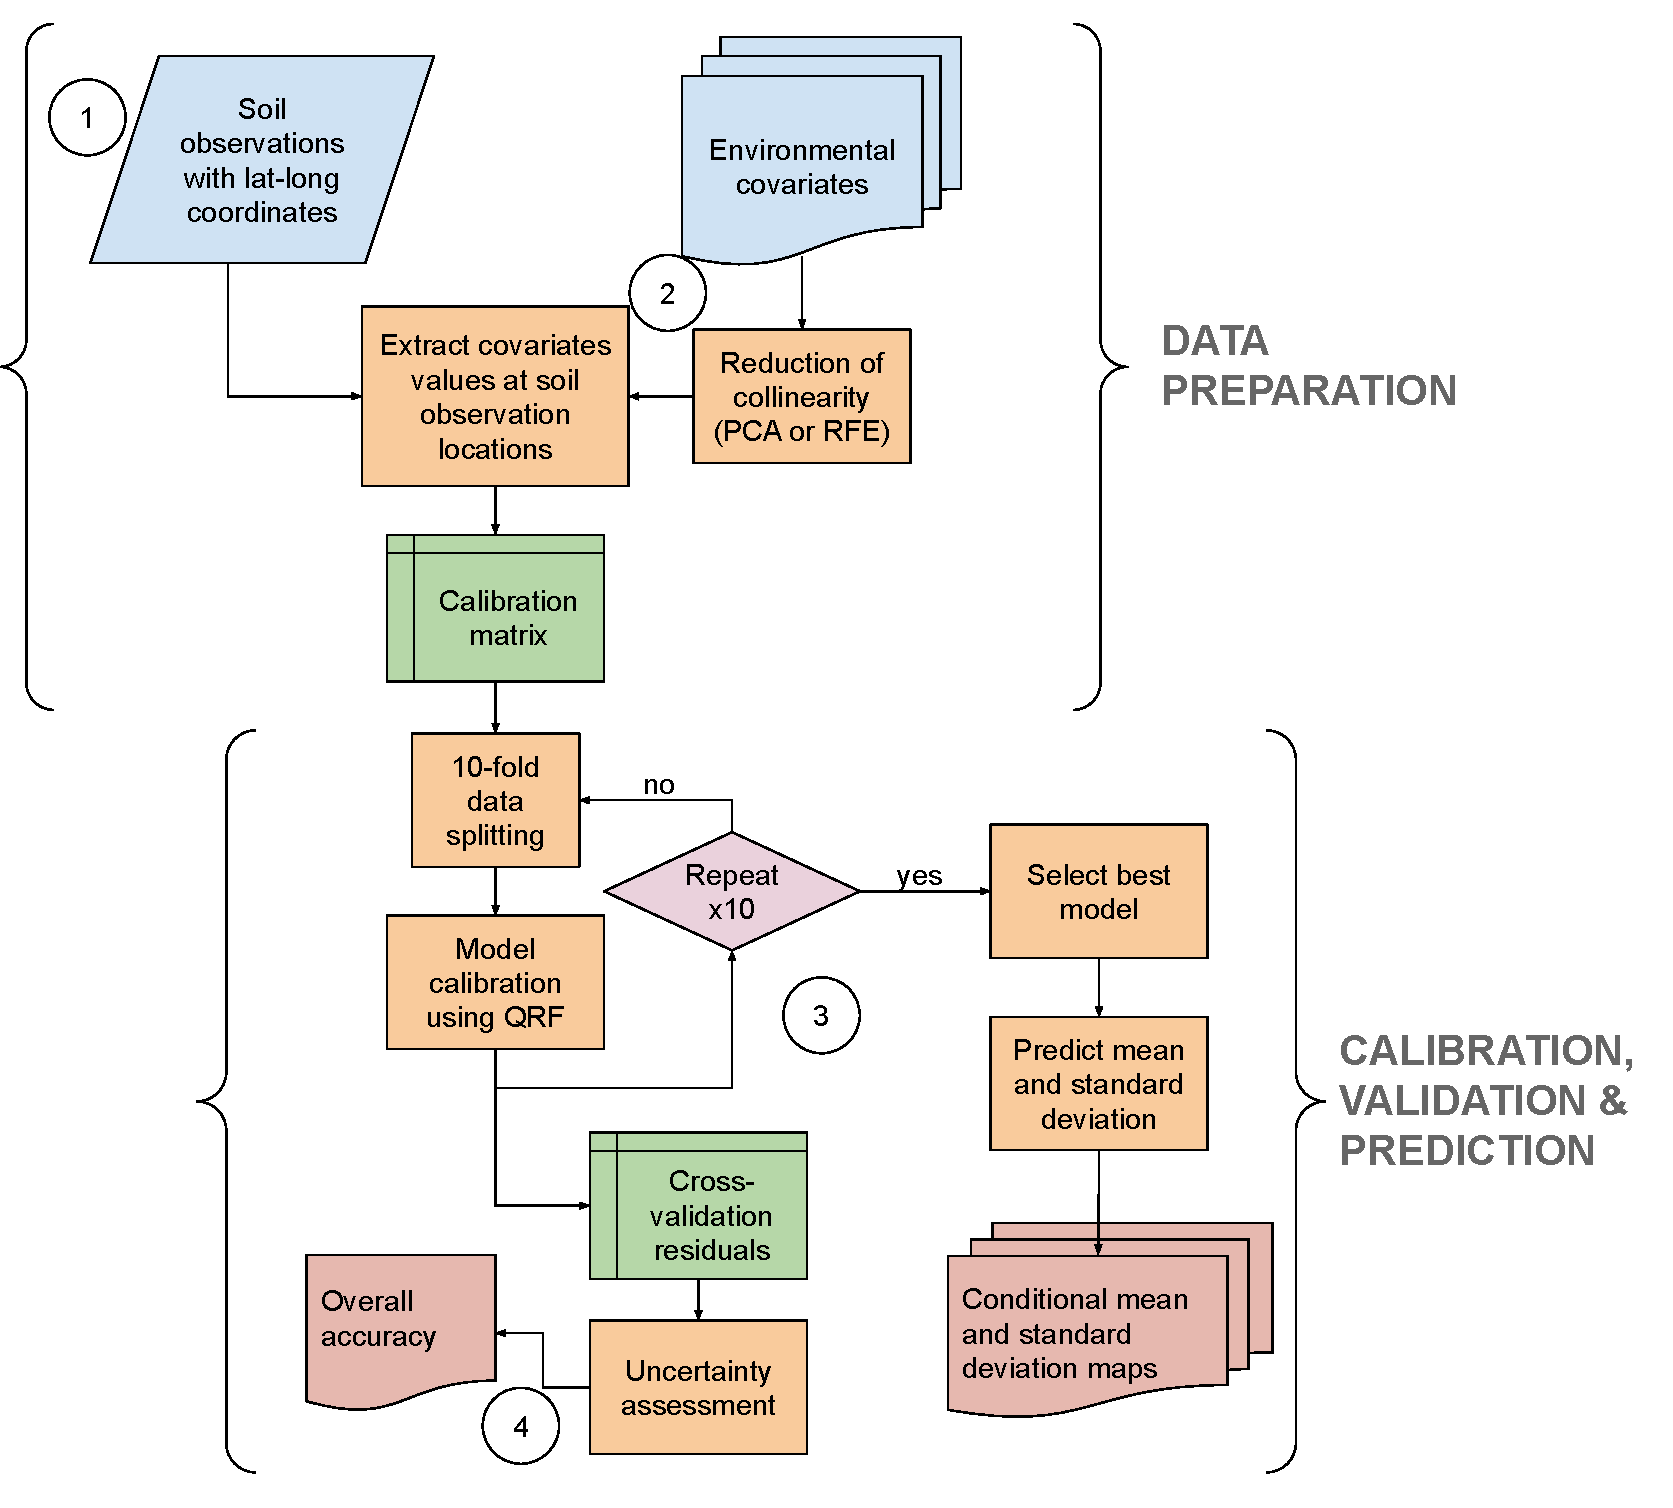
\includegraphics[width=0.9\textwidth]{images/workflow lat-long data.pdf}
  \caption{Digital soil mapping approach for point-support data. Circles are the steps.}
  \label{fig:workflow1}
\end{figure}

\hypertarget{step-1-soil-data-preparation}{%
\chapter{Step 1: soil data preparation}\label{step-1-soil-data-preparation}}

Soil data consist of measurement at a specific geographical location, time and soil depth. Therefore, it is necessary to arrange the data following the format shown in Table \ref{tab:data1}.

\begin{table}[htbp]
    \caption{Format example of a soil dataset}
    \scalebox{0.685}{
    \begin{threeparttable}
        \centering
            \begin{tabular}{rrrrrrrrrl}
            \toprule
            Profile ID & Horizon ID & Lat & Long & Year & Top  & Bottom  & Soil property & Value & Lab method\\
            \midrule
            1 & 1\_1 & 12.123456 & 1.123456 & 2018 & 0  & 20 & SOC & 3.4 & W\&B \\
            1 & 1\_2 & 12.123456 & 1.123456 & 2018 & 20 & 40 & SOC & 2.1 & W\&B \\
            2 & 2\_1 & 23.123456 & 2.123456 & 2019 & 0  & 30 & SOC & 2.9 & W\&B\\
            \bottomrule
        \end{tabular}
        \begin{tablenotes}
        \item \footnotesize Profile ID = unique profile identifier; Horizon ID = unique layer identifier; Lat = latitude in decimal degrees; Long = longitude in decimal degrees; Year = sampling year; Top = upper limit of the layer in cm; Bottom = lower limit of the layer in cm; Soil property = name of the soil property; Value = numerical value of the measure; Lab method = name of the laboratory protocol used for measuring the soil property.
        \end{tablenotes}
    \end{threeparttable}
    \label{tab:data1}
    }
\end{table}

Soil data usually require a preprocessing step to solve common issues such as, arranging the data format, fixing soil horizon depth consistency, detecting unusual soil property measurements, among others issues.
Once the original dataset is clean and consistent, data harmonisation is needed to produce synthetic horizons (such as 0-30 cm layer), as well as to make compatible measurements from different lab methods. Horizon harmonisation will be done with the mass preserving spline function (\protect\hyperlink{ref-Bishop1999}{Bishop, McBratney and Laslett, 1999}; \protect\hyperlink{ref-Malone2009}{Malone \emph{et al.}, 2009}) fitted to each individual soil profile, which requires more than a layer per profile. In the cases of single-layer samples, which is common in sampling for nutrient determination, a pedotransfer function locally calibrated should be applied. Pedotransfer functions will be also required to harmonise the laboratory methods. Experts from GLOSOLAN will provide advice in this regard.

\hypertarget{step-2-environmental-covariates}{%
\chapter{Step 2: environmental covariates}\label{step-2-environmental-covariates}}

\hypertarget{environmental-covariates}{%
\section{Environmental covariates}\label{environmental-covariates}}

The SCORPAN equation (Eq. \ref{eq:scorpan}) refers to the soil-forming factors that determine the spatial variation of soils. However, these factors cannot be measured directly. Instead, proxies of these soil forming factors are used. One essential characteristic of the environmental covariates is that they are spatially explicit, covering the whole study area. Table 2 shows a summary of the environmental covariates that can be implemented under the DSM framework.

\begin{longtable}{p{0.12\textwidth}  p{0.47\textwidth} p{0.20\textwidth} p{0.10\textwidth}}

        \caption{Environmental covariates}\\ 
        \hline
        Factor & Description & Code & Resolution \endfirsthead 
        \hline
        Temp-erature & Mean air temperature (annual) & bio1 & 1000 \\
        & Mean daily temperature of warmest month & bio5 & 1000 \\
        & Mean daily temperature of coldest month & bio6 & 1000 \\ 
        \hline
        Precipi-tation & Total precipitation (annual) & bio12 & 1000 \\
        & Mean precipitation of wettest month & bio13 & 1000 \\
        & Mean precipitation of driest month & bio14 & 1000 \\
        & Mean monthly precipitation of wettest quarter & bio16 & 1000 \\
        & Mean monthly precipitation of driest quarter & bio17 & 1000 \\ 
        \hline
        Evapotransp-iration & Mean monthly PET & pet\_penman\_mean & 1000 \\
        & Minimum monthly PET & pet\_penman\_min & 1000 \\
        & Range monthly PET & pet\_penman\_range & 1000 \\
        & Maximum monthly PET & pet\_penman\_max & 1000 \\ 
        \hline
        Wind & Minimum monthly wind speed & sfcWind\_min & 1000 \\
        & Maximum monthly wind speed & sfcWind\_max & 1000 \\
        & Range monthly wind speed & sfcWind\_range & 1000 \\ 
        \hline
        Growing season & Number of days with mean daily air temperature  10 °C & ngd10 & 1000 \\ 
        \hline
        Vegetation Indices & NDVI (MOD13Q1), mean March-May from 2000-2022 & ndvi\_030405\_mean & 250 \\
        & NDVI (MOD13Q1), mean June-August from 2000-2022 & ndvi\_060708\_mean & 250 \\
        & NDVI (MOD13Q1), mean September-November from 2000-2022 & ndvi\_091011\_mean & 250 \\
        & NDVI (MOD13Q1), mean December-February from 2000-2022 & ndvi\_120102\_mean & 250 \\
        & NDVI (MOD13Q1), standard deviation March-May from 2000-2022 & ndvi\_030405\_sd & 250 \\
        & NDVI (MOD13Q1), standard deviation June-August from 2000-2022 & ndvi\_060708\_sd & 250 \\
        & NDVI (MOD13Q1), standard deviation September-November from 2000-2022 & ndvi\_091011\_sd & 250 \\
        & NDVI (MOD13Q1), standard deviation December-February from 2000-2022 & ndvi\_120102\_sd & 250 \\ 
        \hline
        FPAR & Fraction of photosynthetically active radiation (FPAR) (MOD15A2H), mean March-May from 2000-2022 & fpar\_030405\_mean & 500 \\
        & Fraction of photosynthetically active radiation (FPAR) (MOD15A2H), mean June-August from 2000-2022 & fpar\_060708\_mean & 500 \\
        & Fraction of photosynthetically active radiation (FPAR) (MOD15A2H), mean September-November from 2000-2022 & fpar\_091011\_mean & 500 \\
        & Fraction of photosynthetically active radiation (FPAR) (MOD15A2H), mean December-February from 2000-2022 & fpar\_120102\_mean & 500 \\
        & Fraction of photosynthetically active radiation (FPAR) (MOD15A2H), standard deviation March-May from 2000-2022 & fpar\_030405\_sd & 500 \\
        & Fraction of photosynthetically active radiation (FPAR) (MOD15A2H), standard deviation June-August from 2000-2022 & fpar\_060708\_sd & 500 \\
        & Fraction of photosynthetically active radiation (FPAR) (MOD15A2H), standard deviation September-November from 2000-2022 & fpar\_091011\_sd & 500 \\
        & Fraction of photosynthetically active radiation (FPAR) (MOD15A2H), standard deviation December-February from 2000-2022 & fpar\_120102\_sd & 500 \\ 
        \hline
        LST & Land Surface Temperature Day (MOD11A2), mean March-May from 2000-2022 & lstd\_030405\_mean & 1000 \\
        & Land Surface Temperature Day (MOD11A2), mean June-August from 2000-2022 & lstd\_060708\_mean & 1000 \\
        & Land Surface Temperature Day (MOD11A2), mean September-November from 2000-2022 & lstd\_091011\_mean & 1000 \\
        & Land Surface Temperature Day (MOD11A2), mean December-February from 2000-2022 & lstd\_120102\_mean & 1000 \\
        & Land Surface Temperature Day (MOD11A2), standard deviation March-May from 2000-2022 & lstd\_030405\_sd & 1000 \\
        & Land Surface Temperature Day (MOD11A2), standard deviation June-August from 2000-2022 & lstd\_060708\_sd & 1000 \\
        & Land Surface Temperature Day (MOD11A2), standard deviation September-November from 2000-2022 & lstd\_091011\_sd & 1000 \\
        & Land Surface Temperature Day (MOD11A2), standard deviation December-February from 2000-2022 & lstd\_120102\_sd & 1000 \\ 
        \hline
        NDLST & Normalised Difference between LST Day and LST Night (MOD11A2), mean March-May from 2000-2022 & ndlst\_030405\_mean & 1000 \\
        & Normalised Difference between LST Day and LST Night (MOD11A2), mean June-August from 2000-2022 & ndlst\_060708\_mean & 1000 \\
        & Normalised Difference between LST Day and LST Night (MOD11A2), mean September-November from 2000-2022 & ndlst\_091011\_mean & 1000 \\
        & Normalised Difference between LST Day and LST Night (MOD11A2), mean December-February from 2000-2022 & ndlst\_120102\_mean & 1000 \\
        & Normalised Difference between LST Day and LST Night (MOD11A2), standard deviation March-May from 2000-2022 & ndlst\_030405\_sd & 1000 \\
        & Normalised Difference between LST Day and LST Night (MOD11A2), standard deviation June-August from 2000-2022 & ndlst\_060708\_sd & 1000 \\
        & Normalised Difference between LST Day and LST Night (MOD11A2), standard deviation September-November from 2000-2022 & ndlst\_091011\_sd & 1000 \\
        & Normalised Difference between LST Day and LST Night (MOD11A2), standard deviation December-February from 2000-2022 & ndlst\_120102\_sd & 1000 \\ 
        \hline
        SWIR & Black-sky albedo for shortwave broadband (MCD43A3), mean June-August from 2000-2022 & swir\_060708\_mean & 500 \\ 
        \hline
        Snow cover & MODIS Snow Cover (MOD10A1) mean & snow\_cover & 500 \\ 
        \hline
        Land cover & Dynamic World 10m near-real-time (NRT) Land Use/Land Cover (LULC) dataset. Mean estimated probability of complete coverage by trees & trees & 250 \\
        & Dynamic World 10m near-real-time (NRT) Land Use/Land Cover (LULC) dataset. Mean estimated probability ofcomplete coverage by shrub and scrub & shrub\_and\_scrub & 250 \\
        & Dynamic World 10m near-real-time (NRT) Land Use/Land Cover (LULC) dataset. Mean estimated probability of complete coverage by flooded vegetation & flooded\_vegetation & 250 \\
        & Dynamic World 10m near-real-time (NRT) Land Use/Land Cover (LULC) dataset. Mean estimated probability of complete coverage by grass & grass & 250 \\
        & Dynamic World 10m near-real-time (NRT) Land Use/Land Cover (LULC) dataset. Mean estimated probability of complete coverage by bare & crop & 250 \\ 
        \hline
        Terrain & Profile curvature & curvature & 250 \\
        & Downslope curvature & downslopecurvature & 250 \\
        & Uplslope curvature & upslopecurvature & 250 \\
        & Deviation from Mean Value & dvm & 250 \\
        & Deviation from Mean Value & dvm2 & 250 \\
        & Elevation & elevation & 250 \\
        & Melton Ruggedness Number & mrn & 250 \\
        & Negative openness & neg-openness & 250 \\
        & Possitive openness & por-openness & 250 \\
        & Slope & slope & 250 \\
        & Topographic position index & tpi & 250 \\
        & Terrain wetness index & twi & 250 \\
        & Multirresolution of valley bottom flatness & vbf & 250 \\
        \hline
\label{tab:covs}
\end{longtable}

Apart from the environmental covariates mentioned in Table \ref{tab:covs}, other types of maps could also be included, such as Global Surface Water Mapping Layers and Water Soil Erosion from the Joint Research Centre (JRC). At national level there may be very significant covariates that could complement or replace the covariates of Table \ref{tab:covs}.

Since environmental covariates are available at different resolutions and coordinate reference systems (CRS), they have to be harmonised at a common resolution and CRS. The target resolution in GSNmap is 250 m x 250 m, therefore, all covariates were aggregated (from higher to lower resolution) or disaggregated (from lower to higher resolution) to 250 m. This process involved a raster resampling method, which is usually implemented by a bilinear approach for continuous covariates, and by the nearest-neighbour approach for categorical covariates (not included in the current list).

Note that the target resolution of GSNmap has been set at 250 m, which can be considered a moderate resolution for a global layer. However, those countries that require a higher resolution are free to develop higher resolution maps and aggregate the resulting maps to the target resolution of GSNmap for submission.

\hypertarget{reducing-collinearity-in-environmental-covariates}{%
\section{Reducing collinearity in environmental covariates}\label{reducing-collinearity-in-environmental-covariates}}

Multicollinearity is usually present in remote sensing data and terrain attributes. While this was an issue for multiple linear regression models, current models such as random forest can deal with high dimensionality. However, the main reasons to reduce the number of environmental covariates are that a model with fewer predictors can be interpreted more easily, thus extracting new knowledge, redundant information increasing the computational demand, and improve prediction results (\protect\hyperlink{ref-Behrens2014}{Behrens \emph{et al.}, 2014}).

Covariate selection can be done by supervised or unsupervised methods (\protect\hyperlink{ref-Behrens2010}{Behrens \emph{et al.}, 2010}). Supervised methods work on the basis of prediction results, hence they are based on a given dataset. For instance, recursive feature elimination (RFE) in caret R package (\protect\hyperlink{ref-Kuhn2022}{Kuhn, 2022}) provides a tool for selecting covariates according to their predicting contribution. Instead, unsupervised methods are used to reduce the dimensionality of the dataset by removing redundant information without taking into account a particular target variable. Principal component analysis is one of the most widely used for this purpose, however, it does not ensure that specific discriminant features are kept within the main factors (\protect\hyperlink{ref-Behrens2014}{Behrens \emph{et al.}, 2014}). Another drawback of this technique is that model interpretation can be reduced when using factors instead of the original covariates.

\hypertarget{merging-soil-data-and-environmental-covariates}{%
\section{Merging soil data and environmental covariates}\label{merging-soil-data-and-environmental-covariates}}

A calibration dataset consists of soil observations and a matrix of predictors, where each row is a soil observation paired with the values of the corresponding covariates for the given spatial location. Some common issues and solution when merging soil observations and covariates are:

\begin{itemize}
\tightlist
\item
  Mismatch of coordinate reference system (CRS): it requires to convert the CRS of point data to the raster or polygon covariate CRS.
\item
  Categorical covariates: some covariates may be categorical, such as land use/cover, legacy soil maps or geological maps. A common problem in this case is that some classes may not be sampled with any soil observation, causing an error when using the layer for prediction, since the model cannot predict over a class that was not part of the model calibration step. Also, because of the cross-validation procedure, it is advised to have, at least, three soil samples per class for the same reason.
\end{itemize}

\hypertarget{step-3-mapping-continuous-soil-properties}{%
\chapter{Step 3: Mapping continuous soil properties}\label{step-3-mapping-continuous-soil-properties}}

\hypertarget{setting-up-repeated-k-fold-cross-validation}{%
\section{Setting up repeated k-fold cross validation}\label{setting-up-repeated-k-fold-cross-validation}}

Cross validation is one of the most used methods in DSM for assessing the overall accuracy of the resulting maps (Step 8, Figure 3). Since this is implemented along with the model calibration step, we explain the process at this stage.

Cross validation consists of randomly splitting the input data into a training set and a testing set. However, a unique testing dataset can bias the overall accuracy. Therefore, k-fold cross validation randomly splits the data into k parts, using 1/k part of it for testing and k-1/k part for training the model. In order to make the final model more robust in terms of parameter estimations, we include repetitions of this process. The final approach is called repeated k-fold cross-validation, where k will be equal to ten in this process. A graphical representation of the 10-fold cross validation is shown in Figure \ref{fig:cv}. Note that green balls represent the samples belonging to the testing set and yellow balls are samples of the training set. Each row is a splitting step of the 10-folds, while each block (repetitions) represent the repetition step.

\begin{figure}[t]
  \centering
  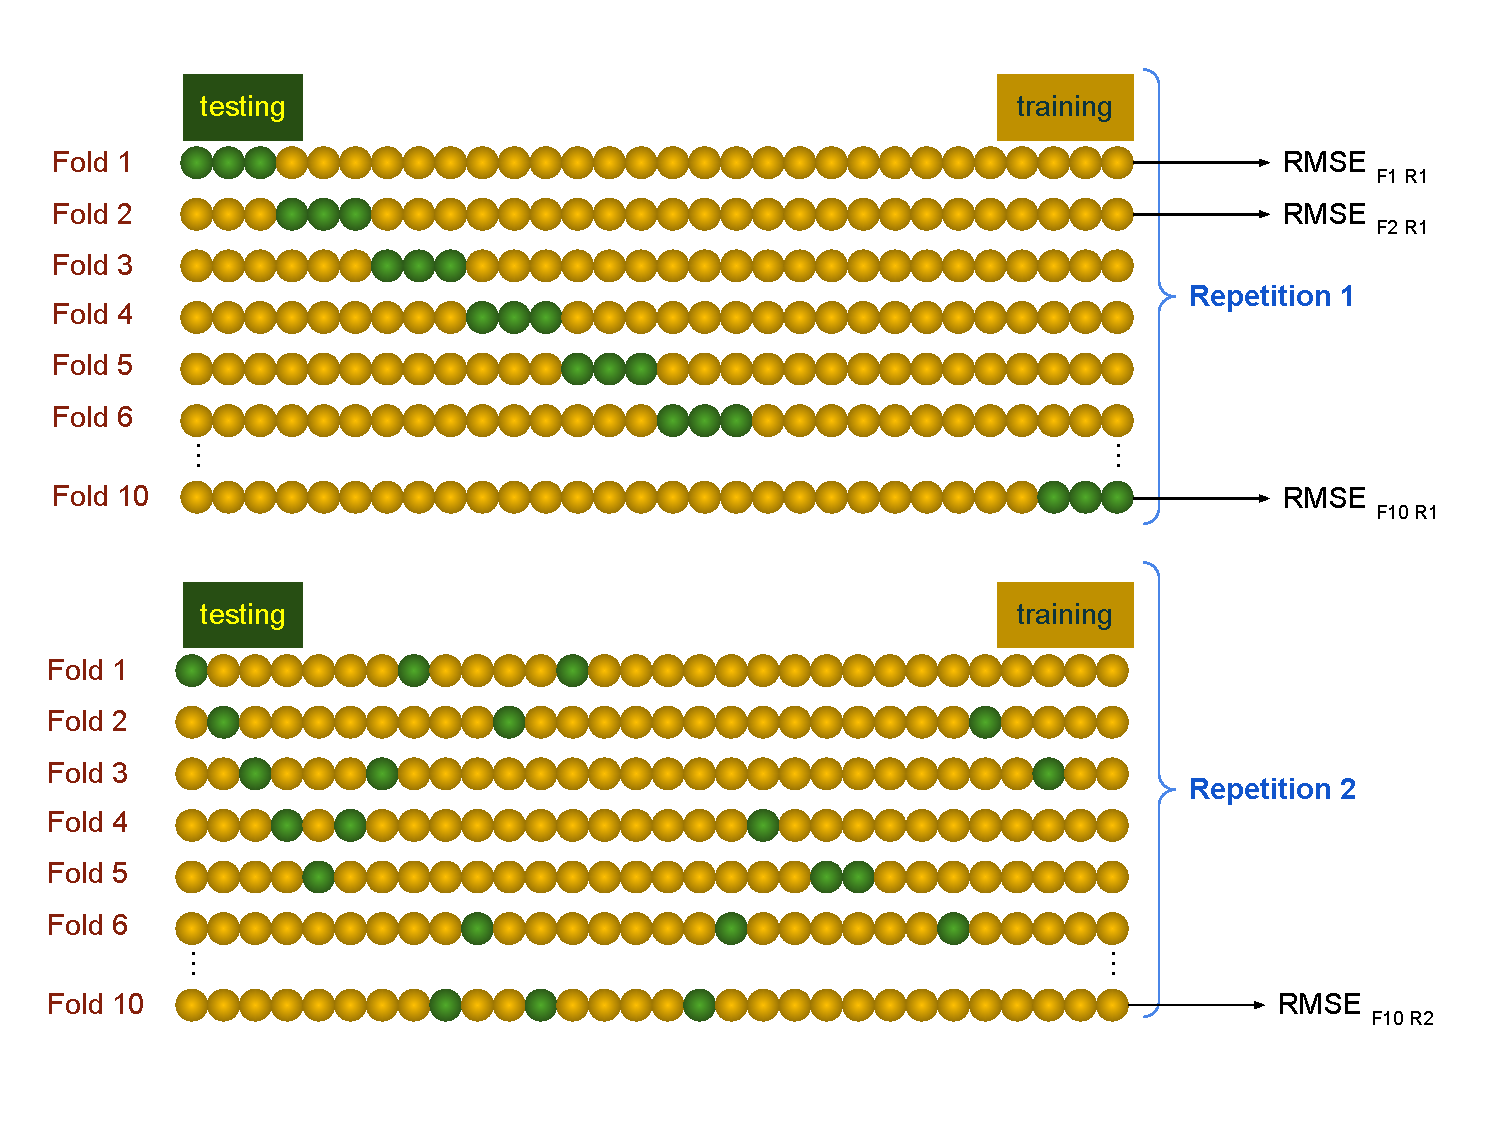
\includegraphics[width=0.9\textwidth]{images/cv.pdf}
  \caption{Schematic representation of the repeated cross-validation process.}
  \label{fig:cv}
\end{figure}

Step 5 in Figure 3 represents the repeated cross-validation, but note that after each single splitting step (the rows in Figure 4) the training data go to model calibration, which will be explained in Step 6 (next Section), and the testing data will be used with the calibrated model to produce the residuals (Step 8, Section 2.2.8).
Repeated cross validation has been nicely implemented in the caret R package (\protect\hyperlink{ref-Kuhn2022}{Kuhn, 2022}), along with several calibration methods.

\hypertarget{model-calibration}{%
\section{Model calibration}\label{model-calibration}}

The model calibration step involves the use of a statistical model to find the relations between soil observations and environmental covariates. One of the most widely used models in DSM is random forest (\protect\hyperlink{ref-Breiman2001}{Breiman, 2001}). Random forest is considered a machine learning method which belongs to the decision-tree type of model. Random forest creates an ensemble of trees using a random selection of covariate. The prediction of a single tree is made based on the observed samples mean in the leaf. The random forest prediction is made by taking the average of the predictions of the single trees. The size of the number of covariates at each tree (mtry) can be fine-tuned before calibrating the model.

Quantile regression forests (QRF, Meinshausen (\protect\hyperlink{ref-Meinshausen2006}{2006})) are a generalisation of the random forest models, capable of not only predicting the conditional mean, but also the conditional probability density function. This feature allows one to estimate the standard deviation of the prediction, as well as the likelihood of the target variable falling below a given threshold. In a context where a minimum level of a soil nutrient concentration may be decisive for improving the crop yield, this feature can play an important role for the GSNmap initiative.

Model calibration will be implemented using the caret package (\protect\hyperlink{ref-Kuhn2022}{Kuhn, 2022}). While we suggest to use QRF, caret provides a large set of models \url{https://topepo.github.io/caret/available-} models.html\#) that might perform better in specific cases. In this regard, it is up to the user to implement a different model, ensuring the product specifications (Section Product Specifications).

\hypertarget{predicting-soil-attributes}{%
\section{Predicting soil attributes}\label{predicting-soil-attributes}}

After calibrating the model, caret will select the best set of parameters and will fit the model using the whole dataset. Then, the final model can be used to predict the target soil properties. The process uses the model and the values of the covariates at target locations. This is generally done by using the same input covariates as a multilayer raster format, ensuring that the names of the layers are the same as the covariates in the calibration dataset. In this step we will predict the conditional mean and conditional standard deviation at each raster cell.

\hypertarget{step-4-uncertainty-assessment}{%
\chapter{Step 4: uncertainty assessment}\label{step-4-uncertainty-assessment}}

\hypertarget{introduction}{%
\section{Introduction}\label{introduction}}

Accuracy assessment is an essential step in digital soil mapping. One aspect of the accuracy assessment has been done in Step 7 by predicting the standard deviation of the prediction, which shows the spatial pattern of the uncertainty. Another aspect of the uncertainty is the estimation of the overall accuracy to measure the model performance. This will be measured using the model residuals generated by caret during the repeated cross validation step.

The residuals produced by caret consist of tabular data with observed and predicted values of the target soil property. They can be used to estimate different accuracy statistics. Wadoux, Walvoort and Brus (\protect\hyperlink{ref-Wadoux2022}{2022}) have reviewed and evaluated many of them. While they concluded that there is not a single accuracy statistic that can explain all aspect of map quality, they recommended the following:
mean prediction error (ME), that estimates the prediction bias;
mean absolute prediction error (MAE) and root mean squared prediction error (RMSE) to estimate the magnitude of the errors; and
model efficiency coefficient (MEC) (\protect\hyperlink{ref-Janssen1995}{Janssen and Heuberger, 1995}) as an estimator of the proportion of variance explained by the model.

While solar diagrams (\protect\hyperlink{ref-Wadoux2022}{Wadoux, Walvoort and Brus, 2022}) are desired, we propose to produce a scatterplot of the observed vs predicted values maintaining the same range and scale for the X and Y axes.

Finally, note that accuracy assessment has been discussed in Wadoux \emph{et al.} (\protect\hyperlink{ref-Wadoux2021}{2021}), since the spatial distribution of soil samples might constrain the validity of the accuracy statistics. This is especially true in cases where the spatial distribution of observations is clustered. The authors recommended creating a kriging map of residuals before using them for assessing the map quality.

\hypertarget{reporting-results}{%
\chapter{Reporting results}\label{reporting-results}}

\hypertarget{compendium-of-r-scripts}{%
\chapter{Compendium of R scripts}\label{compendium-of-r-scripts}}

\hypertarget{references}{%
\chapter*{References}\label{references}}
\addcontentsline{toc}{chapter}{References}

\hypertarget{refs}{}
\begin{CSLReferences}{0}{0}
\leavevmode\vadjust pre{\hypertarget{ref-Behrens2014}{}}%
\textbf{Behrens, T., Schmidt, K., Ramirez-Lopez, L., Gallant, J., Zhu, A.-X. \& Scholten, T.} 2014. Hyper-scale digital soil mapping and soil formation analysis, 213: 578--588. \url{https://doi.org/10.1016/j.geoderma.2013.07.031}

\leavevmode\vadjust pre{\hypertarget{ref-Behrens2010}{}}%
\textbf{Behrens, T., Zhu, A.-X., Schmidt, K. \& Scholten, T.} 2010. Multi-scale digital terrain analysis and feature selection for digital soil mapping, 155: 175--185. \url{https://doi.org/10.1016/j.geoderma.2009.07.010}

\leavevmode\vadjust pre{\hypertarget{ref-Bishop1999}{}}%
\textbf{Bishop, T.F.A., McBratney, A.B. \& Laslett, G.M.} 1999. Modelling soil attribute depth functions with equal-area quadratic smoothing splines, 91: 27--45. \url{https://doi.org/10.1016/s0016-7061(99)00003-8}

\leavevmode\vadjust pre{\hypertarget{ref-Breiman2001}{}}%
\textbf{Breiman, L.} 2001. Random forests. \emph{Machine Learning}, 45(1): 5--32. \url{https://doi.org/10.1023/A:1010933404324}

\leavevmode\vadjust pre{\hypertarget{ref-Hengl2017}{}}%
\textbf{Hengl, T., Leenaars, J.G.B., Shepherd, K.D., Walsh, M.G., Heuvelink, G.B.M., Mamo, T., Tilahun, H., Berkhout, E., Cooper, M., Fegraus, E., Wheeler, I. \& Kwabena, N.A.} 2017. Soil nutrient maps of sub-saharan africa: Assessment of soil nutrient content at 250 m spatial resolution using machine learning, 109: 77--102. \url{https://doi.org/10.1007/s10705-017-9870-x}

\leavevmode\vadjust pre{\hypertarget{ref-Janssen1995}{}}%
\textbf{Janssen, P.H.M. \& Heuberger, P.S.C.} 1995. Calibration of process-oriented models, 83: 55--66. \url{https://doi.org/10.1016/0304-3800(95)00084-9}

\leavevmode\vadjust pre{\hypertarget{ref-Kuhn2022}{}}%
\textbf{Kuhn, M.} 2022. \emph{Caret: Classification and regression training}. (also available at \url{https://CRAN.R-project.org/package=caret}).

\leavevmode\vadjust pre{\hypertarget{ref-Malone2009}{}}%
\textbf{Malone, B.P., McBratney, A.B., Minasny, B. \& Laslett, G.M.} 2009. Mapping continuous depth functions of soil carbon storage and available water capacity, 154: 138--152. \url{https://doi.org/10.1016/j.geoderma.2009.10.007}

\leavevmode\vadjust pre{\hypertarget{ref-McBratney2003}{}}%
\textbf{McBratney, A.B., Santos, M.L.M. \& Minasny, B.} 2003. On digital soil mapping, 117: 3--52. \url{https://doi.org/10.1016/s0016-7061(03)00223-4}

\leavevmode\vadjust pre{\hypertarget{ref-Meinshausen2006}{}}%
\textbf{Meinshausen, Ni.} 2006. Quantile regression forests. \emph{Journal of Machine Learning Research}, 7(6).

\leavevmode\vadjust pre{\hypertarget{ref-Wadoux2021}{}}%
\textbf{Wadoux, A.M.J.-C., Heuvelink, G.B.M., Bruin, S. de \& Brus, D.J.} 2021. Spatial cross-validation is not the right way to evaluate map accuracy, 457: 109692. \url{https://doi.org/10.1016/j.ecolmodel.2021.109692}

\leavevmode\vadjust pre{\hypertarget{ref-Wadoux2022}{}}%
\textbf{Wadoux, A.M.J.-C., Walvoort, D.J.J. \& Brus, D.J.} 2022. An integrated approach for the evaluation of quantitative soil maps through taylor and solar diagrams, 405: 115332. \url{https://doi.org/10.1016/j.geoderma.2021.115332}

\end{CSLReferences}

%\printindex
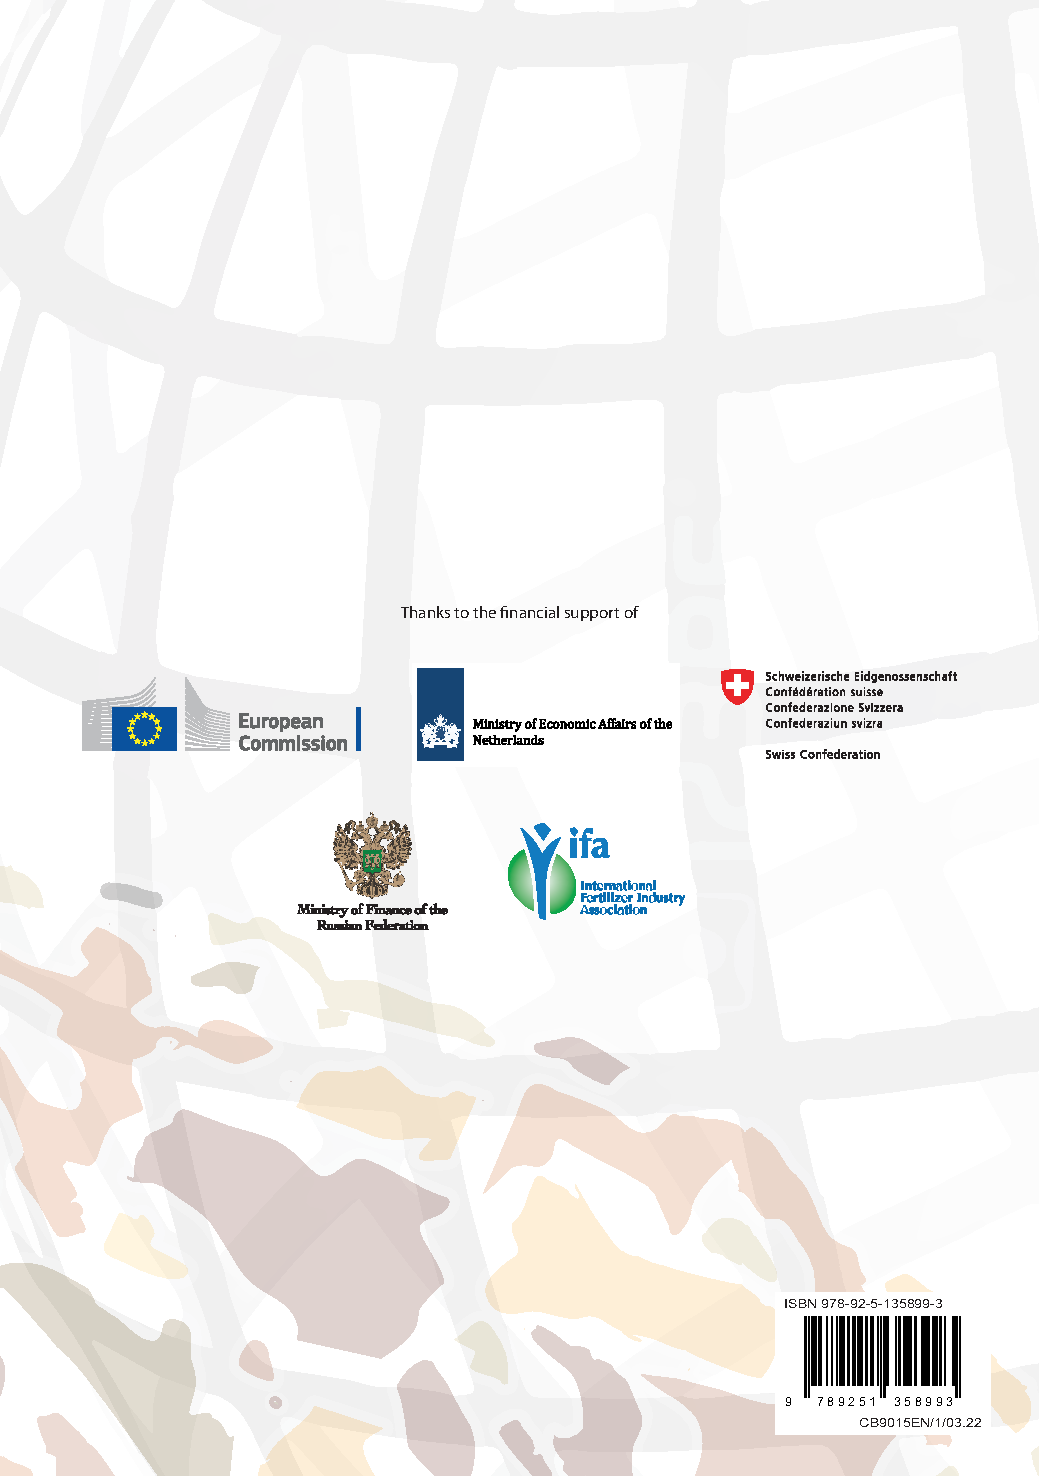
\includepdf{images/backcover.pdf}

\end{document}
